\subsection{PID for CLAS12}
The Particle identification (PID) is the procedure of selecting signal events while
rejecting background events, and is a key step in the data analysis for essentially
all particle physics experiments.
HEP experiments include various approaches from the Bayesian statistical and 
log-likelihood technique \cite{BELLE,HERMES}
to more sophisticated Boosted Decision 
Trees (BDT) \cite{BDT} and Artificial Neural Networks (ANN) \cite{ANN}.

The identification  of the scattered lepton is crucial in electroproduction experiments.
The comprehensive research programme of CLAS12 comprises both physics with semi-inclusive and 
hard exclusive processes, where identification of hadronic particles is also required.
The identification of electrons and hadrons at CLAS12 is based on the detector responses 
of the forward calorimeter (EC), the preshower (PCAL)and the High Threshold 
Cherenkov Counter (HTCC). The hadron identification includes the Low Threshold Cherenkov
Counter (LTCC), central (CTOF) and forward (FTOF) time-of-flight counters.
The particle identification at CLAS12 will be accomplished combining 
the reconstructed vertex, momentum and angles from tracking detectors (FST,BST,DC)
information with responses of 
relevant detector components (HTCC, LTCC, TOF, PCAL, EC).
 One  possible PID scheme
for CLAS12 could be the probability based procedure, when for each particle type a probability
that the measured detector signal was caused by that particle is calculated
by comparing the signal with parent distributions which are the typical 
responses of the different particle types in the detector.

\begin{figure}[htb]
\begin{minipage}[b]{5.0cm}
   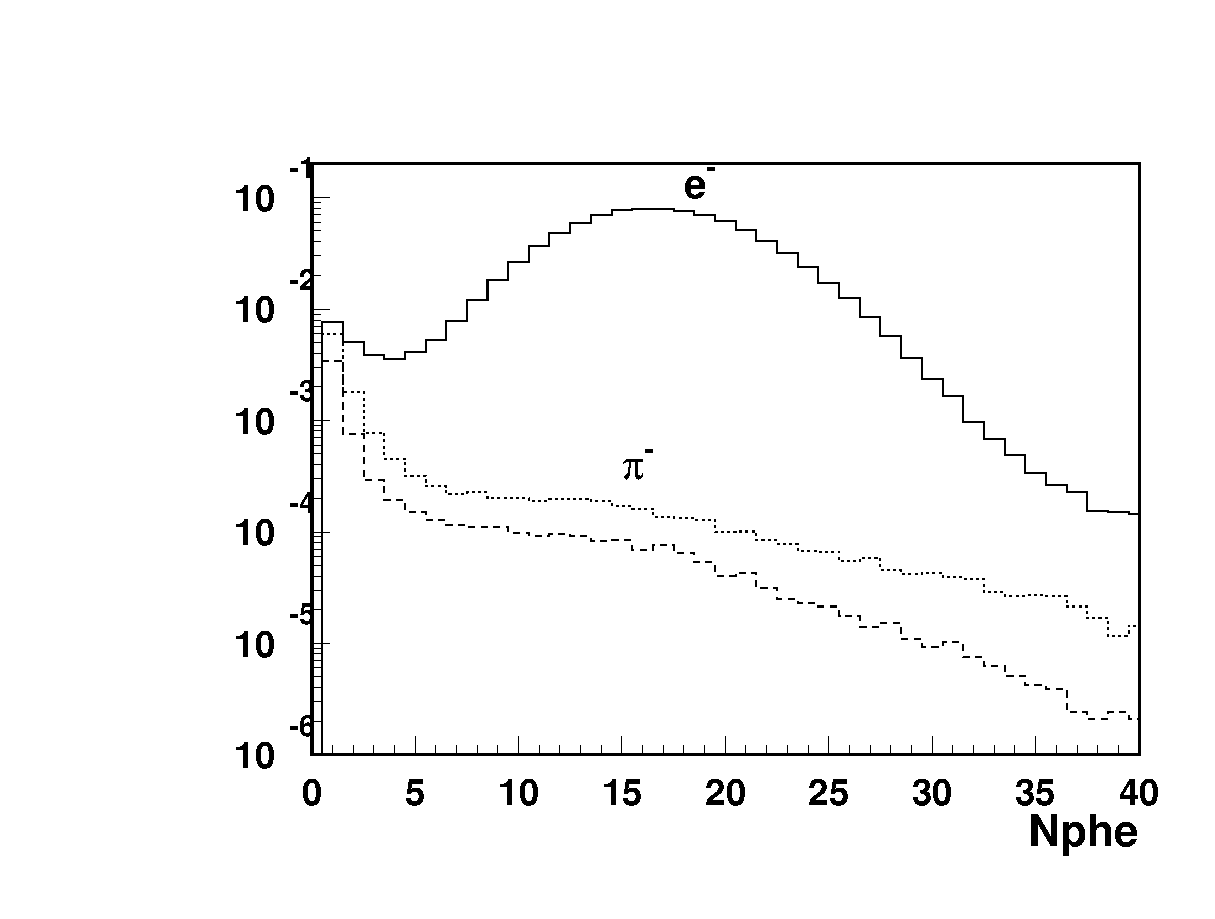
\includegraphics[width=3in]{pid/htccvlas.eps} 
   \end{minipage}
   \begin{minipage}[b]{5.0cm}
 \includegraphics[width=3in]{pid/parentNormPCAL.eps}
 	\end{minipage}
	\begin{minipage}[b]{5.0cm}
	\includegraphics[width=3in]{pid/parentNormECPCAL.eps}
	\end{minipage}
	\caption{\it Parent distributions for $\pi^-$ and electron for the high 
threshold Cherenkov counter (HTCC), the preshower (PCAL) and the sum
of the responses of the preshower and the forward calorimeter (PCAL+EC). The solid lines
are for electrons and dashed for pions. Dotted line shws pions at 2 GeV.
}
\label{fig:parent1}
 \end{figure}



\subsubsection{Probability Analysis}

The probability analysis  based on the extraction of probabilities that 
a measured detector response $E$ was caused by particles of a certain type, $A_i$. This 
conditional probability $P(A_i|E)$ is related through Bayes's theorem to the conditional 
probability  $P(E|A_i)$ that particle of a given type $A_i$ causes a detector response $E$:

\begin{equation}
P(A_i|E)= \frac{P(A_i)\cdot P(E|A_i)}{\sum_{k=1}^n P(A_k)\cdot P(E|A_k)},
\end{equation}

where the sum runs over all particle types $A_k$ an $P(A_i)$ is the probability that 
a particle of type $A_i$ is present in the detector.

The conditional probability $P(E|A_i)$ for a given detector $D$ is equivalent to the 
parent distribution ${\cal L}_D^i$ that depends on the particle type, the detector 
response $E$, and the momentum $p$ of the particle:

\begin{equation}
{\cal L}_D^i \equiv {\cal L}_D^i(E,p,\theta).
\end{equation}

The parent distributions are an intrinsic property of a PID detector
that can be calculated through normalizing the appropriate particle counts as a 
function of the detector response. Eventually the parent distributions will be extracted
from the data collected during the normal operation of the experiment, 
as during the time the detector response may change. 
In the extraction of parent distribution clean samples of certain type of particles
are required, which can be achieved by introducing very tight cuts on other PID detectors,
while analyzing the certain PID detector. CLAS12, compared to other DIS experiments, where
that technique was used, provides a unique possibility to use exclusive processes, where
the PID is defined from the exclusivity condition, to produce the parent distributions.
In the design stage 
we use the parent distributions obtained from the GEANT simulation of the relevant detectors.
The parent distributions are normalized to 1 and give the probability for a certain
type of particle to give a response E. Some typical parent distributions 
for pions and electrons in certain
bins of momentum (p=4 GeV) and polar angle ($\theta$=15 degree)  obtained from GEANT
simulaton of CLAS12 \cite{HTCC,PCAL} are shown on 
Fig.\ref{fig:parent1}. 


The probability $P(A_i)$ is given by the normalized flux $\phi^i$ which depends on the 
momentum $p$ and the scattering angle $\theta$ of the particle:

\begin{equation}
P(A_i)= \phi^i \equiv   \phi^i(p,\theta)
\end{equation}

The conditional probability ${\cal P}^i\equiv P(A_i|E)$, that a certain particle 
type has been observed, can be determined from the detector response using Bayes's 
theorem if the parent distributions and the particle fluxes are known. The parent
distributions can be extracted from collected data or theoretical models.

The probability for a certain particle (ex. electron) in a detector D is given by:
\begin{equation}
{\cal P}_D^e = \frac{{\cal L}_D^e}{\Phi {\cal L}_D^h+{\cal L}_D^e},
\end{equation}

where $\Phi\equiv \phi^h/\phi^e$ is the flux ratio of hadrons and electrons. In order
not to rely on determination of individual fluxes, one can use the logarithm of the ratio
of the electron and hadron probabilities for a given detector:

\begin{equation}
log_{10} \frac{{\cal P}_D^e}{{\cal P}_D^h}= log_{10} 
\frac{{\cal L}_D^e}{\Phi {\cal L}_D^h}=log_{10}\frac{{\cal L}_D^e}{{\cal L}_D^h}-log_{10}\Phi
\end{equation}

The final discrimination between the particle types will be accomplished by combining 
the probabilities from all relevant PID detectors:

\begin{equation}
PID=log_{10}(\prod_D \frac{{\cal L}_D^e}{{\cal L}_D^h})=\sum_D (log_{10} 
\frac{{\cal L}_D^e}{{\cal L}_D^h})
\end{equation}

To improve the efficiency of the detection system while retaining good particle separation
different combinations of PID detectors could be combined in set of PID observables.
In addition to one-dimensional PID cuts, this will allow two and more dimensional 
scatter-plots for the PID variables.

Similar procedure could be used for hadron identification involving the low threshold
Cherenkov counter (LTCC) and forward TOF for forward tracks and central TOF for large angle
track identification.

The identification of electrons and hadrons  can be improved, if a sensible estimate 
of the flux factors is available. The flux ratio is calculated in number of bins in 
momentum and polar angle. The ratio of fluxes of pions and electrons as a function of momentum 
for different polar angles calculated using SLAC parameterization \cite{SLAC} 
is plotted on Fig. \ref{fig:flux}.

\begin{figure}[htb]
  \centering
   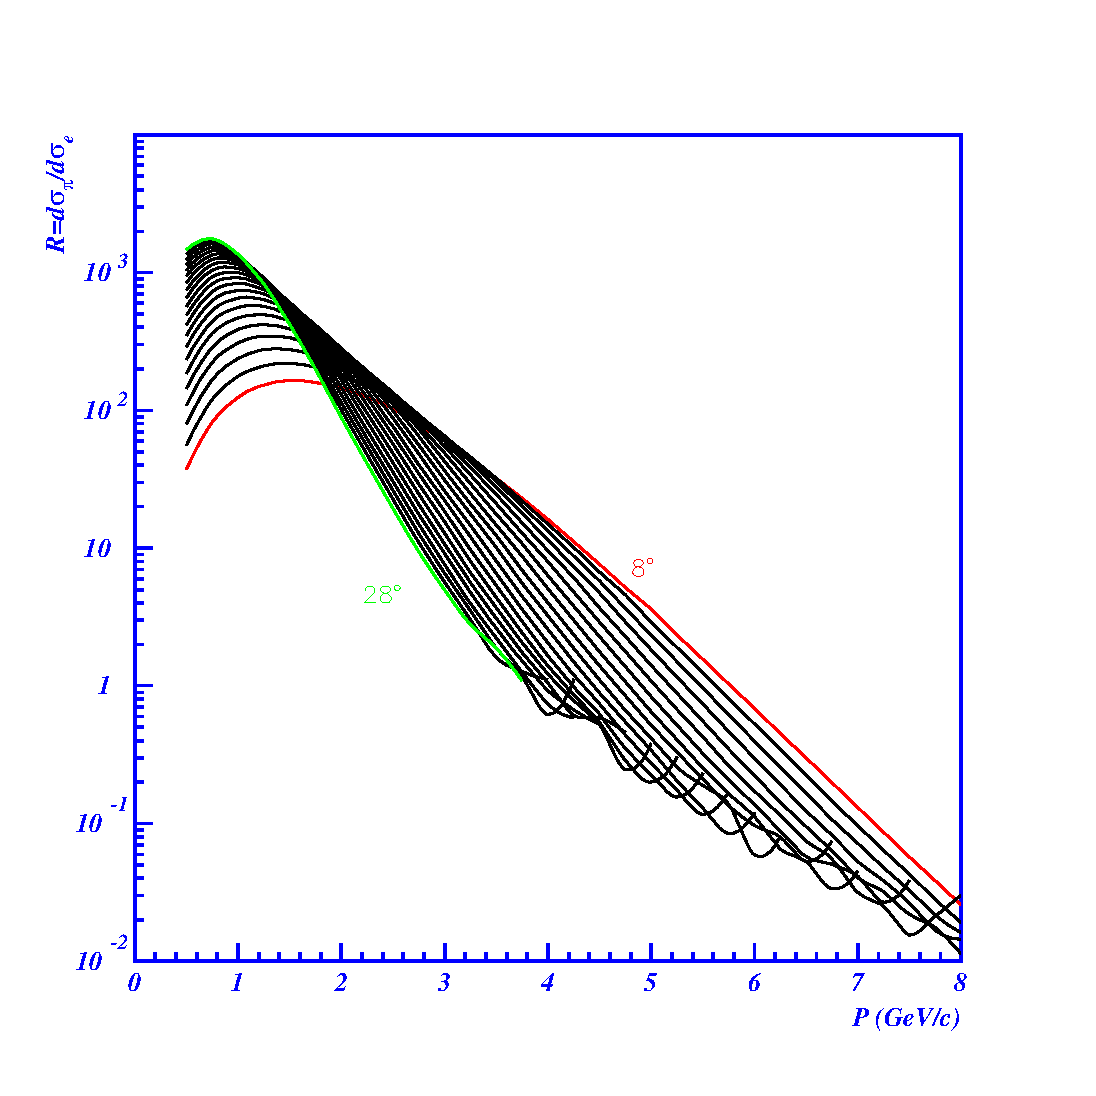
\includegraphics[width=6in]{pid/pi_e_csratio.eps}
\caption{\it The ratio of fluxes of pions and electrons as a function of momentum 
for different polar angles.
}
\label{fig:flux}
\end{figure}

In reality the fluxes are not known precisely and will also have significant dependence
on the initial trigger. The flux could be extracted from the date using an iterative
procedure starting with some reasonable initial flux, or even a uniform flux. The data
analysis with some initial flux will yield a new flux which goes as input for the next
iteration. This procedure typically converges in less than ten iterations \cite{HERMES,HERMES1}

Three variables are generally used to describe the performance of the particle 
identification scheme: the hadron rejection factor (HRF), the electron efficiency 
and the contamination of the
electron sample defined as the percentage of hadrons in the electron sample.
The PITHIA generator and CLAS12 fast Monte-Carlo program (FASTMC) will be initially 
used to test the PID chain and analyse the PID performance.
The electron reconstruction (and identification) efficiency as a function
of contamination is shown on Figure \ref{fig:effic}.

\begin{figure}[htbp] %  figure placement: here, top, bottom, or page
   \centering
   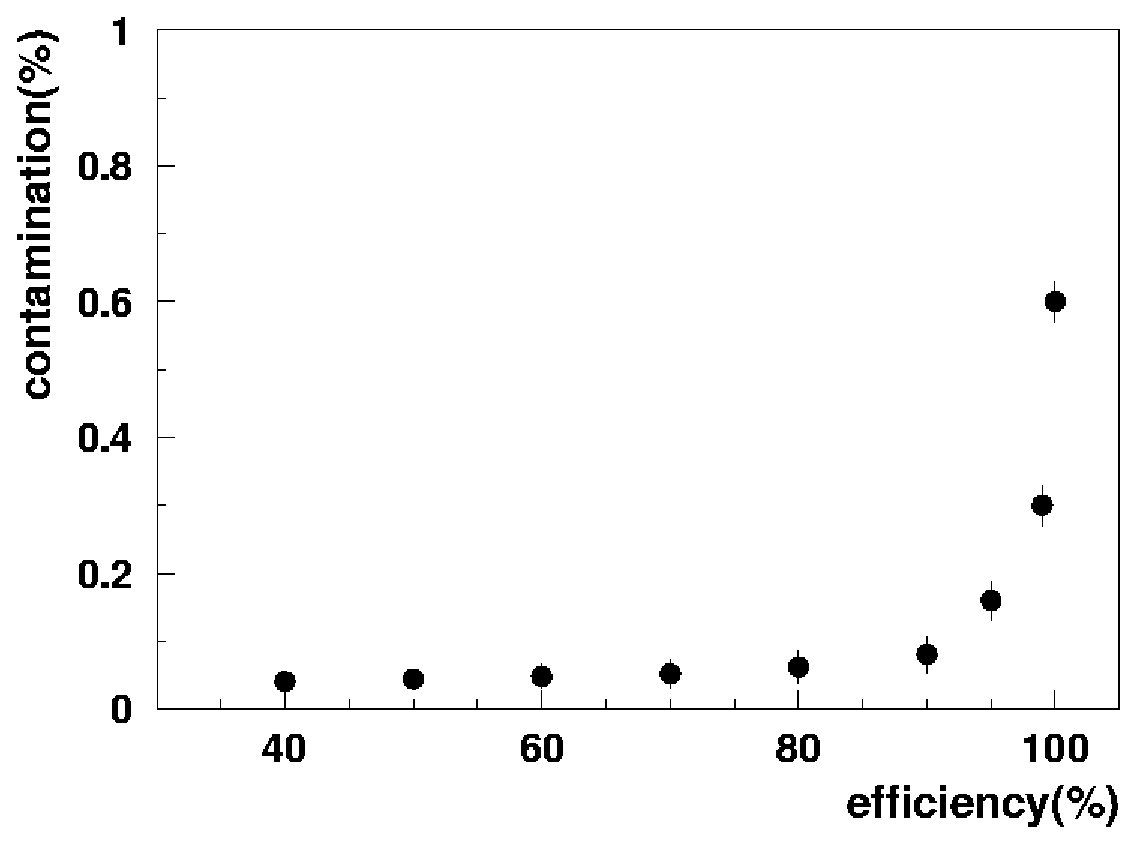
\includegraphics[width=6in]{pid/effic.eps} 
  \caption{\it The hadron contamination as a function of the electron efficiency.
The 2 sets show 2 different trigger conditions.
}
\label{fig:effic}
\end{figure}



  
